\chapter{Diseño de la solución}
\label{chap:diseño}

En este capítulo describiremos la estrategia que seguimos para refactorizar el bucle MAPE-K \foreign{english}{Lite}. Como comentamos en la introducción, nuestro objetivo era adaptarlo a entornos \foreign{english}{cloud}. Esto implica transformarlo de un servicio monolítico a un sistema distribuido basado en microservicios. Se trata de un cambio arquitectónico importante. Por ello, queríamos seguir una estrategia ingenieril que tenga en cuenta las particularidades del sistema.

Comenzaremos justificando la elección de este estilo arquitectónico y describiendo los beneficios que esperábamos obtener. A continuación, detallaremos nuestro diseño y explicaremos cómo se dividió la funcionalidad del bucle en microservicios. Después, presentaremos algunos de los mecanismos de comunicación más populares y comentaremos cuáles elegimos para conectar nuestros componentes. Finalmente, presentaremos la estructura final de nuestra arquitectura.

\section{¿Por qué usar microservicios?}
\label{sec:por-que-microservicios}

Una de las decisiones clave que tomamos durante el desarrollo de este trabajo fue elegir el estilo arquitectónico a emplear. Dado que queremos adaptar el bucle de control a entornos en la nube, será imprescindible que esté preparado para ellos. Optamos por las \textbf{arquitecturas basadas en microservicios} porque son uno de los pilares de las aplicaciones \foreign{english}{cloud native}. \cite{gannonCloudNativeApplications2017} Gracias a este estilo, obteníamos una serie de beneficios que consideramos vitales para extender el bucle MAPE-K.

El más evidente fue poder \textbf{independizar la implementación} de los servicios. Si fuera necesario, podríamos emplear tecnologías distintas para cada uno. Distintas plataformas o lenguajes de programación que nos permitan ofrecer la funcionalidad requerida. Incluso podríamos contar con implementaciones alternativas de algunos componentes. Estos podrían ofrecer diferentes estrategias de la misma funcionalidad: distintos planificadores, módulos de análisis, etc.

También vimos muy importante el desarrollar \textbf{servicios \foreign{english}{plug \& play}}. Al añadir o eliminar componentes podríamos cambiar las capacidades de adaptación del sistema en tiempo de ejecución. Sin necesidad de pararlo en ningún momento. Por ejemplo, al desplegar un nuevo conjunto de reglas de adaptación se dotaría al bucle de capacidades para gestionar otros aspectos de los recursos.

Por otro lado, facilitaría \textbf{escalar la capacidad computacional} de cada servicio de forma independiente. Si uno en concreto estuviera recibiendo más peticiones que los demás, podemos limitarnos a desplegar una nueva instancia de este componente. No sería necesario desplegar el bucle completo. Esto nos permitirá aprovechar mejor los recursos disponibles.

Finalmente, nos ayudaría a desacoplar el bucle de los componentes específicos para gestionar una solución autoadaptativa determinada. Así, en un futuro, podríamos aprovechar la misma infraestructura para manejar varias soluciones simultáneamente. Esto se conoce como multicliente o \textbf{\foreign{english}{multi-tennancy}}. Como tiene importantes implicaciones a nivel de seguridad y gestión de los datos de los distintos clientes \cite{aljahdaliMultitenancyCloudComputing2014}, en este trabajo no profundizaremos más allá de separar los componentes.

Optar por un estilo arquitectónico determinado tiene un precio. Conlleva una serie de desventajas que no podremos ignorar. Aun así, se consideró que los beneficios las compensaban. Entre ellas, la más importante es un \textbf{aumento en la complejidad} del sistema. \cite{newmanBuildingMicroservicesDesigning2021} Pasamos de trabajar con un solo servicio monolítico a tener que gestionar varios más pequeños.

A nivel de diseño, esto afectará a la \textbf{comunicación entre servicios}. Como ya no se ejecutan dentro del mismo proceso, deberán comunicarse a través de la red. Más adelante veremos que esta no es infalible. \cite{jausovecFallaciesDistributedSystems2020} Pueden ocurrir retrasos para entregar los mensajes o directamente fallar la conexión. Por tanto, necesitaremos plantear bien cómo y cuándo deberán contactar entre ellos. Lo ideal es que sean lo más independientes posible, ya que cada dependencia es un potencial punto de fallo.

Otros aspectos que se verán afectados serán la \textbf{operación y el despliegue del sistema}. Para su correcto funcionamiento tendremos que monitorizar y gestionar cada una de sus piezas. Como una sola petición puede desencadenar llamadas a otros servicios, requeriremos de soluciones de monitorización y \foreign{english}{logging} más avanzadas. \cite{parkerDistributedTracingPractice2020} Sin una buena solución de \textbf{observabilidad} puede ser muy difícil de depurar los errores o analizar su impacto.

\section{Distribución de los componentes}

Una vez elegido el estilo arquitectónico, el siguiente paso fue identificar qué servicios compondrían nuestra arquitectura. Por suerte, partíamos de un sistema existente bien documentado. Conocíamos el rol de cada uno de sus elementos y sus requisitos. Nos quedaba entonces determinar cómo agrupar estos elementos en servicios. ¿Cómo definimos las fronteras entre cada uno de ellos? ¿Qué componentes debe abarcar cada microservicio?

Para ello nos guiamos por unas pautas para dividir aplicaciones monolíticas. \cite{newmanBuildingMicroservicesDesigning2021} Los servicios que definamos deben presentar \textbf{alta cohesión} en su funcionalidad. Es decir, siempre que sea posible debemos agrupar los componentes relacionados en un mismo servicio. De lo contrario, acabarían muy acoplados entre sí. No serían realmente independientes y necesitarían comunicarse constantemente. En caso de que uno de ellos falle, el resto no podría operar con normalidad.

Por este motivo, una de las primeras decisiones que tomamos fue \textbf{separar cada etapa del bucle a su propio servicio}. Entre ellas existe una división funcional bien definida y pueden operar con cierta independencia. Además, como el conocimiento es compartido entre todas las etapas, también tendría su propio microservicio. Esto nos reportaría los beneficios que comentamos en la sección anterior como las implementaciones independientes y la posibilidad de escalar su capacidad de cómputo individualmente.

La siguiente división que consideramos fue \textbf{separar del bucle de control los componentes específicos de las soluciones manejadas}. Se trata de los monitores, reglas y demás elementos que conocen el dominio de la solución. Actualmente se despliegan en el mismo proceso que el bucle. En caso de querer cambiar alguno, tendríamos que redesplegarlo entero. Extrayéndolos a servicios independientes, el bucle se volverá agnóstico a las soluciones manejadas. En tiempo de ejecución podremos añadir o eliminar estos componentes, sin que afecte a su funcionamiento.

En la figura \ref{fig:mape-k-microservices} mostramos la arquitectura resultante de estas divisiones de funcionalidad. \textbf{Cada elemento es un tipo distinto de microservicio}. Las sondas y los efectores son un caso especial. Podrán desarrollarse como microservicios o como elementos empotrados en el recurso manejado. Dependerá de si tenemos control o no sobre la implementación del recurso.

\begin{figure}[htb]
  \centering
  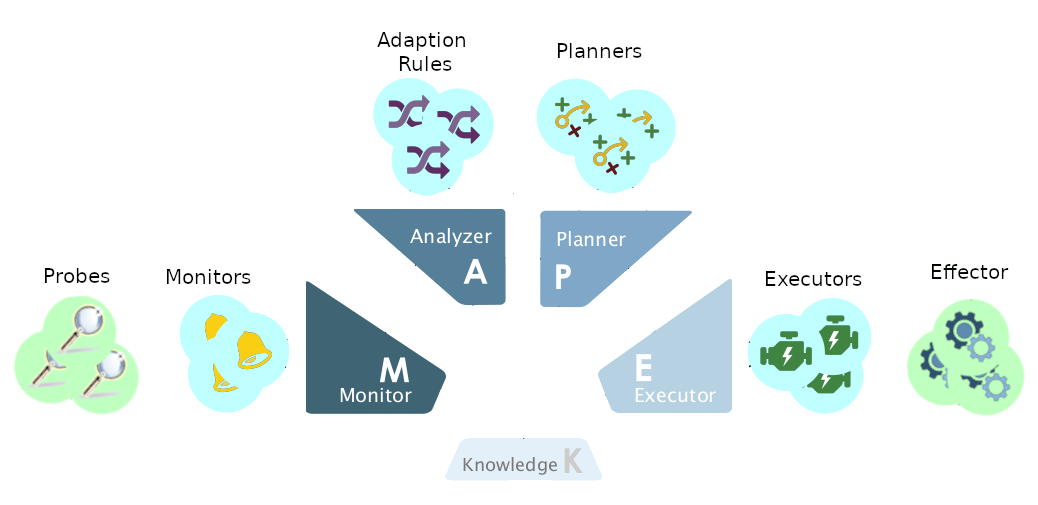
\includegraphics[scale=0.5]{cap_diseño/images/componentes-segunda-division}
  \caption{Diagrama con los microservicios que conforman nuestra arquitectura distribuida.}
  \label{fig:mape-k-microservices}
\end{figure}

\section{Conectando los servicios}

El siguiente problema al que nos enfrentamos está relacionado con la comunicación. Si dividimos estos componentes en microservicios, ¿cómo deberían comunicarse? Hay que tener en cuenta que estos pueden estar desplegados y replicados en distintas máquinas. No podemos asumir que están en el mismo \foreign{english}{host}.

Para elegir los mecanismos de comunicación, investigamos algunos de los estilos arquitectónicos existentes. Finalmente, nos decantamos por las \textbf{arquitecturas de servicios jerarquizados}. Estas nos permitían explotar la separación entre el bucle de control y los recursos manejados. En concreto, nos inspiramos en el estilo arquitectónico C2 (\emph {components and connectors})\cite{taylorComponentMessagebasedArchitectural1996a, UCISoftwareArchitecture}.

\subsection{Jerarquías de microservicios: Arquitectura C2 y arquitectura limpia}

Este estilo organiza sus elementos en jerarquías o capas. Un componente se ubicará en un nivel determinado en base a su nivel de abstracción respecto al entorno de ejecución. En las capas inferiores se encuentran aquellos más externos, los más ''acoplados al mundo real''. Por ejemplo, las interfaces de usuario estarían en esta capa. Por otro lado, en las capas superiores se encuentran los servicios con mayor abstracción. Este sería el caso de las reglas de negocio de un programa. No hay ninguna restricción en cuanto al número de capas, podemos contar con cuantas sea necesario.

\pagebreak

En cuanto a la comunicación, un componente solo puede contactar con sus vecinos inmediatos (en una capa superior o inferior). Limitando su contacto con otras capas limitamos su alcance y su conocimiento sobre el resto del sistema. Así evitamos que se acople al resto de componentes más de lo necesario. Además, dentro de un mismo nivel no pueden contactar entre ellos. Según la dirección de la comunicación, se emplean mecanismos distintos (figura \ref{fig:C2-arch-example}):

\begin{itemize}
  \item \textbf{Peticiones} (\emph{requests}): Se trata de solicitudes a un servicio concreto para que ejecute una acción. Un componente se comunica con un vecino en una capa superior. La petición viaja de ''abajo a arriba'' en cuanto al nivel de abstracción. Por ejemplo, una petición de un usuario a la interfaz gráfica entraría en esta categoría.

  \item \textbf{Notificaciones}: Un componente envía un mensaje hacia abajo en la jerarquía, sin especificar un receptor. Todos los servicios que estén por debajo lo recibirán y decidirán si tratarlo o no. Esto evita que nuestro componente se acople a ellos. Se puede emplear para comunicar eventos que puedan ser de interés al resto. Un ejemplo sería notificar al resto de servicios sobre la creación de un nuevo usuario.
\end{itemize}

\begin{figure}[htb]
  \centering
  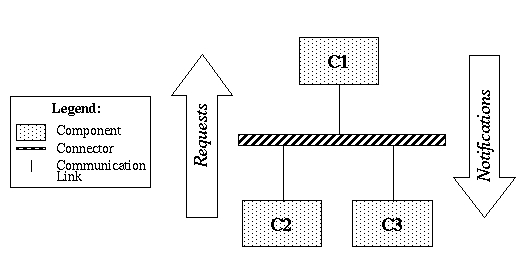
\includegraphics[scale=0.45]{cap_diseño/images/c2SampleArch}
  \caption[Ejemplo del estilo arquitectónico C2 (\emph{Components and Connectors})]{Ejemplo del estilo arquitectónico C2 (\emph{Components and Connectors}). \cite{UCISoftwareArchitecture}}
  \label{fig:C2-arch-example}
\end{figure}

Basándonos en este estilo definimos las capas de nuestro sistema. Esto nos permitió organizar los microservicios en jerarquías, lo que nos ayudaría a definir las reglas de nuestra arquitectura. Distinguimos cuatro niveles, de menor a mayor nivel de abstracción:

\begin{itemize}
  \item \textbf{Nivel del recurso manejado}: En este nivel se encuentra el recurso manejado. También se encuentran los elementos que nos permiten interactuar con él: las sondas y efectores. Hacen de intermediarios entre el recurso y el resto del bucle.

  \item \textbf{Nivel de solución}: En esta capa se encuentran los componentes del bucle específicos para una solución autoadaptativa: monitores, reglas de adaptación, etc. No los incluimos en el mismo nivel que las sondas y efectores porque deben comunicarse con ellas. Estos elementos mantienen una dependencia con el propio bucle de control.

  \item \textbf{Nivel del bucle}: Aquí se encuentran los servicios de las etapas del bucle: monitorización, análisis, planificación y ejecución. Esta capa es agnóstica al dominio de los recursos manejados. Además, actúa como intermediario entre los servicios de la solución y el conocimiento, limitando su acceso. Por ejemplo, ningún servicio salvo los monitores deberían poder modificarlo.

  \item \textbf{Conocimiento}: Es la capa más interna y la base de nuestra arquitectura. No depende de ningún otro componente, por lo que tiene el mayor nivel de abstracción. Todos los componentes del nivel del bucle dependen de ella para funcionar.

\end{itemize}

Habiendo definido esta jerarquía, vimos ciertas similitudes con arquitecturas \foreign{english}{domain driven}, como \foreign{english}{Clean Architecture}. \cite{martinChapter22Clean2018a} En ella, el sistema se organiza en base a una \textbf{regla de dependencia}: <<\emph{la dependencia entre los componentes solo puede apuntar hacia dentro, hacia políticas de alto nivel}>>. Es decir, la arquitectura se organiza en \textbf{capas concéntricas}. En el centro se encuentra el dominio, con el mayor nivel de abstracción. Este no tiene dependencias con ninguna capa exterior. Por otro lado, cada capa más externa requiere de componentes de la capa a la que envuelve.

Basándonos en la descripción anterior, optamos por representar nuestra arquitectura como \foreign{english}{knowledge driven}. \cite{taylorSoftwareArchitectureFoundations2009} Nuestra capa central será la del conocimiento (amarilla). A partir de ahí, cada nivel superior dependería de aquella a la que envuelve: el bucle al conocimiento (rojo), la solución al bucle (verde), y la del recurso manejado a la solución (azul). En la figura \ref{fig:clean-mapek-architecture} mostramos el resultado. Las flechas negras representan las peticiones; y las moradas, las notificaciones.

\begin{figure}[htb]
  \centering
  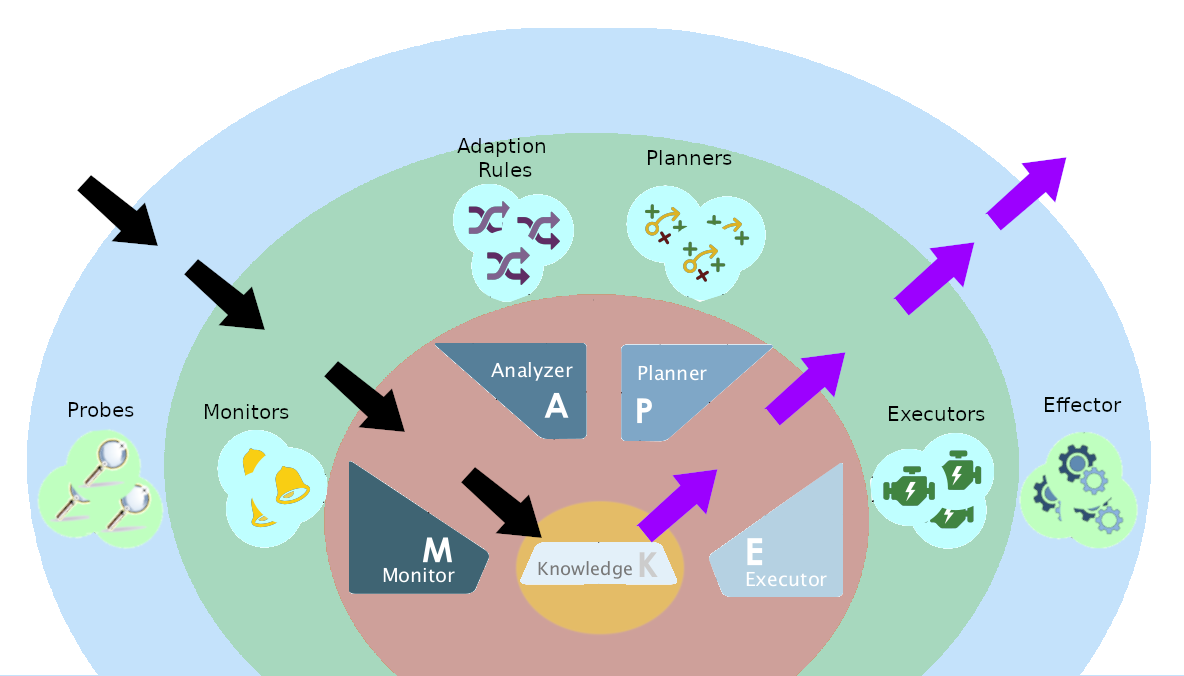
\includegraphics[scale=0.45]{cap_diseño/images/jerarquia-componentes}
  \caption[Representación de nuestra propuesta arquitectónica. Inspirado en Arquitectura Limpia (\emph{Clean Architecture}).]{Representación de nuestra propuesta arquitectónica. Inspirado en Arquitectura Limpia (\emph{Clean Architecture}). \footnotemark }
  \label{fig:clean-mapek-architecture}
\end{figure}

\footnotetext{Basada en imagen de arquitectura limpia obtenida de: \url{https://threedots.tech/post/ddd-cqrs-clean-architecture-combined/}}

\subsection{Definiendo los mecanismos de comunicación}

Como comentamos antes, nos inspiramos en los mecanismos de comunicación descritos por C2: las peticiones y notificaciones. Pero, durante nuestra etapa de prototipado, nos dimos cuenta de que estos no cubren todas nuestras necesidades. Hay dos casos que no están contemplados: la comunicación del módulo de análisis con el planificador, y la del planificador con el ejecutor. El problema estaba en que ambos componentes se encuentran en la misma capa. Como dependen del conocimiento para funcionar, no podíamos moverlos a una superior para emplear las notificaciones.

Requeríamos entonces de un tercer patrón de comunicación. Detectamos que este debería de ser dirigido: los mensajes van destinados a un tipo de componente específico. Y, como los elementos están en el mismo nivel, no queremos que se acoplen entre ellos. Surgió entonces la idea de utilizar las peticiones asíncronas, una combinación de los dos patrones existentes. Lo presentamos a continuación junto al resto de patrones de comunicaciones que empleamos:

\begin{itemize}
  \item \textbf{Peticiones síncronas}: Comunicaciones síncronas dirigidas a un servicio determinado. Un servicio contacta con otro con una petición o comando, y espera al resultado. Sólo están permitidas desde servicios de una capa más externa a un servicio en la capa interior adyacente.

  \item \textbf{Notificaciones}: Comunicaciones asíncronas no dirigidas. El servicio publica un evento que potencialmente recibirán todos los servicios en la capa externa adyacente. El cliente lo envía y continua su ejecución, sin esperar una respuesta.

  \item \textbf{Peticiones asíncronas}: Comunicaciones asíncronas dirigidas a un servicio determinado. Ideal para solicitar peticiones de trabajo asíncronas: se envían y el destinatario lo procesará cuando pueda. El cliente continuará su ejecución, sin esperar respuesta. Este mecanismo de comunicación solo está permitido entre elementos del mismo nivel.

\end{itemize}

\subsection{Conectores}

Una vez determinados los mecanismos de comunicación, comenzamos la búsqueda de los conectores para implementarlos. Seguimos entonces la estrategia descrita en \cite{taylorSoftwareArchitectureFoundations2009}. Esta consiste en investigar las necesidades de comunicación entre componentes y, a partir de sus requisitos, determinar el \textbf{tipo de conector adecuado}. Sabiendo que hemos optado por una arquitectura distribuida, la elección se simplifica: los servicios pueden estar desplegados en máquinas distintas, por lo que el paso de mensajes será a través de la red.

Debido a esto, no recurrimos a la taxonomía que lista \cite{mehtaTaxonomySoftwareConnectors2000}. En su lugar optamos por consultar las estrategias de comunicación habituales para sistemas distribuidos descritas en \cite{newmanBuildingMicroservicesDesigning2021}. Se trata de cuatro mecanismos distintos: Invocación a métodos remotos (\foreign{english}{Remote Procedure Call}), APIs REST, consultas con GraphQL o \foreign{english}{brokers} de mensajería.

Todas estas tecnologías siguen el principio de \textbf{\foreign{english}{smart endpoints and dumb pipes}} (servicios inteligentes y conductos tontos) \cite{lewisMicroservices14}. Se trata de mecanismos de comunicación ligeros, como HTTP, sin mucha lógica asociada para regularla. Se limitan a ser simples conductos que transmiten los mensajes entre servicios. En su lugar, será el emisor será el responsable de gestionarla. Por ejemplo, implementando políticas de reintento o gestionando el enrutamiento de mensajes.

Para elegir los conectores evaluamos las tecnologías mediante un análisis de \foreign{english}{trade-offs}. A continuación, detallamos las ventajas y desventajas que detectamos de cada uno.

\subsubsection{Tipos de conectores}

\textbf{Invocación de métodos remotos} o (\foreign{english}{\textbf{Remote Procedure Call}}): Este patrón se basa en el estilo cliente-servidor. Un servidor expone una serie de funciones que el cliente puede invocar mediante peticiones a través de la red. \cite{newmanBuildingMicroservicesDesigning2021} Estas peticiones incluyen el nombre de la función a ejecutar y sus parámetros. Al finalizar la ejecución, el servidor puede devolver un resultado, si lo hubiera. Existen varios protocolos que implementan este mecanismo como gRPC o SOAP.

En la programación orientada a objetos suele emplearse una evolución de RPC: el paradigma de \textbf{objetos distribuidos}. \cite{tanenbaumChapter10Distributed2007} Este permite al programa cliente interactuar con objetos que se encuentran en servidores remotos como si se encontraran localmente. Se implementa mediante objetos que actúan como \foreign{english}{proxies}, abstrayendo al cliente de la llamada al servidor.

Los \foreign{english}{proxies} ofrecen una interfaz para que el cliente invoque sus métodos localmente. Por debajo, estos realizan una llamada al servicio remoto donde se encuentra realmente. El servidor remoto procesa la petición y nos devolverá un resultado. En la figura \ref{fig:rpc-distributedobjects} incluimos un diagrama de este mecanismo.

Los \foreign{english}{proxies} o (\foreign{english}{stubs} en la terminología de RPC) suelen generarse a partir de un contrato que define qué operaciones ofrecen los objetos. Por ejemplo: SOAP con WDSL, gRPC; o en el caso de objetos distribuidos, Java RMI.

\begin{figure}[htb]
  \centering
  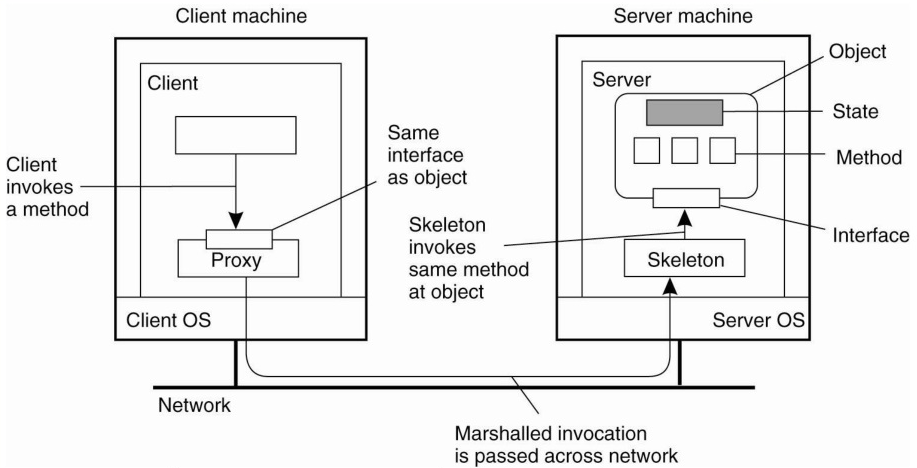
\includegraphics[scale=1.5]{cap_diseño/images/rpc-distributedobjects}
  \caption[Funcionamiento del sistema de objetos distribuidos.]{Funcionamiento del sistema de objetos distribuidos. Obtenido de \cite{tanenbaumChapter10Distributed2007}.}
  \label{fig:rpc-distributedobjects}
\end{figure}

\begin{itemize}
  \item \textbf{Ventajas}:
  \begin{itemize}
    \item El servidor puede ofrecer todo tipo de operaciones a sus clientes. No estamos limitados por un estándar.

    \item Permite distribuir la carga de procesamiento del sistema. Esto puede ayudar para escalar la aplicación.

    \item \textbf{Comunicación síncrona}: Es un mecanismo ideal para comunicaciones síncronas. En ellas, el cliente requiere la respuesta del servicio para poder continuar con su procesamiento.

    \item \textbf{Comunicación asíncrona}: Si el cliente no requiere de una respuesta del servidor, puede enviar el mensaje y continuar con su ejecución. Esta estrategia es conocida como \foreign{english}{fire and forget} (disparar y olvidar).

    \item (\emph{Objetos distribuidos}) Se abstrae al cliente de la interacción con un servidor remoto. Esto facilita su implementación. Al estar tipado, es más sencillo construir las peticiones.

  \end{itemize}

  \item \textbf{Desventajas}:
  \begin{itemize}
    \item \textbf{Dirigida}: Necesitamos conocer de antemano la ubicación del servidor al que queremos hacer una petición.

    \item Dificulta la integración con otras aplicaciones. Cada servicio ofrecerá sus propias funciones. No están estandarizadas.

    \item (\emph{Objetos distribuidos}) Tendremos que actualizar el cliente con cada cambio en el esquema del servidor.

    \item (\emph{Objetos distribuidos}) No se puede abstraer completamente al cliente de las llamadas a través de la red. Pueden darse errores que no ocurrirían durante una invocación de un método sobre un objeto local. Por ejemplo, que el servidor no esté disponible. \cite{jausovecFallaciesDistributedSystems2020}

    \item (\emph{Objetos distribuidos}) Sistemas como Java RMI son específicos para una plataforma concreta. n este caso, Java. Perderemos flexibilidad en cuanto a qué otras tecnologías podemos emplear en nuestra arquitectura. \cite{newmanBuildingMicroservicesDesigning2021}
  \end{itemize}
\end{itemize}

\textbf{\emph{Representational State Transfer} (REST)}: Este mecanismo está basado en RPC, pero con ciertas restricciones adicionales. \cite{taylorSoftwareArchitectureFoundations2009} Sigue también el modelo cliente-servidor. Su concepto principal son los \textbf{recursos}: cualquier elemento sobre el que el servicio pueda ofrecernos información. Estos deben tener asociados un identificador único (una URI). \cite{richardsonRESTfulWebServices2007} Ejemplos de recursos podrían ser las entidades del dominio que gestiona nuestro servicio: usuarios, publicaciones\dots

Las acciones que podemos ejecutar sobre los recursos (leer, crear, actualizar, \dots) las define el protocolo de comunicación sobre el que se implemente. Gracias a esto, la interfaz que ofrecen es \textbf{uniforme}. Solo cambia el ``esquema de los datos``, los tipos de recursos que sirven a los clientes. Esto facilita enormemente la integración con otros servicios. \cite{nallyRESTVsRPC2018} La implementación más habitual es sobre el protocolo HTTP (\foreign{english}{Hypertext Transfer Protocol}). Este define métodos estandarizados como \texttt{GET} para las lecturas, \texttt{PUT} para las actualizaciones, etc.

Otra de las pautas que dicta el estilo es que el servidor no puede mantener el estado de las sesiones de la aplicación (deben ser \textbf{\foreign{english}{stateless}}). Esto significa que cada petición debe poder procesarse de forma independiente. Esto permitirá por un lado que el servidor sea más eficiente, ya que no necesita recordar todos los datos de las sesiones en curso. Por otro lado, si nuestro servicio está replicado, cualquier instancia podrá atender la petición.

\begin{itemize}
  \item \textbf{Ventajas}:

  \begin{itemize}
    \item \textbf{\foreign{english}{Stateless}}: El servidor no mantiene el estado de la sesión del cliente. Esto permite que cada petición sea independiente de las demás.

    \item \textbf{Escalable}: Como las sesiones deben ser \foreign{english}{stateless}, podremos replicar nuestro servicio. Las distintas instancias puedan atender las peticiones que surjan durante una misma sesión.

    \item \textbf{API Uniforme}: Los métodos que exponen estos servicios están estandarizados y son sencillos. Un servidor solo debe implementar unos pocos métodos estándar que consumirán los clientes. Esto mejora significativamente la \textbf{interoperabilidad}.

    \item \textbf{Comunicación síncrona}: Es un mecanismo ideal para el patrón \foreign{english}{request-response}. En ellas, el cliente requiere la respuesta del servicio para poder continuar con su procesamiento.

    \item \textbf{Generación de clientes}: De forma similar a RPC, podemos generar clientes para facilitar la comunicación con APIs REST. Lo explicaremos con más detalle en la sección \ref{chap:OpenAPI} cuando hablemos de OpenAPI.
  \end{itemize}

  \item \textbf{Desventajas}:

  \begin{itemize}
    \item \textbf{Dirigida}: Necesitamos conocer de antemano la ubicación del servidor al que queremos hacer una petición.

    \item \textbf{Rendimiento}: El rendimiento es peor comparado con mecanismos RPC binarios. El tamaño de un mensaje HTTP serializado en XML o JSON es mayor que si estuviera en un formato binario.

    \item \textbf{API Uniforme}: Hay operaciones complejas que pueden ser difíciles de representar con los métodos ofrecidos por el protocolo de comunicación. Pueden requerir más tiempo de diseño, o incluso, ser implementados como métodos RPC (que no siguen el estilo REST).
  \end{itemize}
\end{itemize}

\textbf{GraphQL}\footnote{Página oficial: \url{https://graphql.org/}}: Es protocolo de consultas para APIs. Sigue también el estilo cliente - servidor. El servidor expone un \foreign{english}{endpoint} que permite consultar los datos de la aplicación en forma de \textbf{grafo}. Cada \textbf{nodo} tiene asociado un \textbf{esquema de datos}. Este describe sus propiedades y relaciones con otros. Partiendo de un esquema determinado, podemos realizar consultas que naveguen este grafo. También permite el uso de filtros.

Dota de enorme \textbf{flexibilidad} a los clientes. Con una sola consulta son capaces de recuperar toda la información que consideren relevante. Se evita el \textbf{\foreign{english}{over-fetching}}, recuperar datos irrelevantes. \cite{porcelloLearningGraphQLDeclarative2021} Esto ha provocado que empiece a ganar popularidad frente al estilo REST para realizar consultas complejas. \cite{britoRESTVsGraphQL2020} En REST, estamos limitados a los esquemas de datos de las vistas que ofrezca un recurso. No podemos modificarlos mediante consultas. Incluso, es posible que requiramos de varias llamadas distintas a la API para construir la misma respuesta que en GraphQL.

\begin{itemize}
  \item \textbf{Ventajas}:

  \begin{itemize}
    \item \textbf{Consultas más expresivas}: Nos permite definir consultas tan complejas como necesitemos.

    \item \textbf{Rendimiento}: Es ideal para entornos donde queremos optimizar el uso de red. Esto es gracias a que se reduce la cantidad de llamadas a la API y podemos obtener solo la información relevante.

    \begin{itemize}
      \item Esto lo hace \textbf{ideal para móviles}.
    \end{itemize}

  \end{itemize}

  \item \textbf{Desventajas}:

  \begin{itemize}
    \item \textbf{Solo permite lecturas}: Es un lenguaje de consultas. No tiene comandos que permitan escrituras.

    \item \textbf{Problemas de rendimiento}: Los clientes pueden hacer consultas muy pesadas que penalicen el rendimiento de la base de datos sobre la que opera nuestro servicio.
  \end{itemize}
\end{itemize}

\textbf{\foreign{english}{Brokers} de mensajería}: Es un mecanismo de \textbf{comunicación asíncrona} muy popular. En él, contamos con un servicio que actúa como intermediario de la comunicación, el \textbf{\foreign{english}{broker}}. \cite{newmanBuildingMicroservicesDesigning2021} Este nos permite \textbf{desacoplar} a los participantes. \cite{korabUnderstandingMessageBrokers2017} El emisor de un mensaje no necesita conocer detalles de los destinatarios: su dirección, el número de instancias, si están activos en este momento, etc. Sólo necesita conocer el formato del mensaje, las colas o temas asociados; y enviárselo al \foreign{english}{broker}. Este se encargará de enrutarlo.

Uno de los conceptos más característicos de este estilo son las \textbf{colas de mensajería}. Se trata de colecciones FIFO (\foreign{english}{first in, first out}) donde el \foreign{english}{broker} almacena los mensajes destinados a un servicio \textbf{consumidor}. Cada vez que se añada un mensaje nuevo, el consumidor será notificado. Este podrá ir procesándolos secuencialmente, sin necesidad de saturarse. Las colas nos permiten implementar varias estrategias de comunicación: colas de trabajo, \foreign{english}{publish-suscribe}, híbrida\dots

Tomemos por ejemplo las \textbf{colas de trabajo}. \cite{royChapterMessagePatterns2017} Esta estrategia nos permite implementar comunicaciones asíncronas punto a punto (dirigidas). Es ideal para casos en los que necesitamos que un mensaje llegue sólo una vez a un destinatario determinado. \cite{ibmcorporationWhatAreMessage2020} Por ejemplo, para enviar peticiones de trabajo que pueden ser costosas de procesar. Para enviarlas, el emisor sólo necesita conocer el nombre de la cola de mensajería correspondiente y usar el formato de mensaje apropiado. No requiere conocer ningún otro detalle. En la figura \ref{fig:work-queues} mostramos un ejemplo con un productor (P) que envía el mensaje a una cola con dos consumidores (C1 y C2) a la escucha de esta.

\begin{figure}[htb]
  \centering
  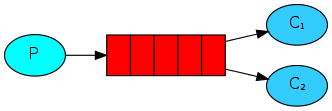
\includegraphics[scale=0.65]{cap_diseño/images/work-queues}
  \caption[Representación de las colas de trabajo. Ejemplo de comunicación asíncrona dirigida.]{Representación de las colas de trabajo. Ejemplo de comunicación asíncrona dirigida. \footnotemark }
  \label{fig:work-queues}
\end{figure}

\footnotetext{Imagen obtenida de: \url{https://www.rabbitmq.com/tutorials/tutorial-two-dotnet.html}}

Otra estrategia que podemos implementar es \textbf{\foreign{english}{publish-suscribe}}. Esta sirve para implementar comunicación \foreign{english}{broadcast}. \cite{royChapterMessagePatterns2017} Se basa en el uso de temas o \textbf{\foreign{english}{topics}}, categorías de mensajes. En base a ellas, los servicios consumidores pueden suscribirse a las que le resulten de interés. Un servicio (el productor) enviará un mensaje al \foreign{english}{broker}, indicando que pertenece a un tema determinado. El \foreign{english}{broker} recibe el mensaje y se encarga de enrutarlo a las colas de todos los consumidores suscritos a él. \cite{rabbitmqPublishSubscribeDocumentation} En la figura \ref{fig:publish-subscribe} tenemos un ejemplo. El mensaje ''A'' llega a todos los servicios suscritos a al tema ''Topic''.

\begin{figure}[htb]
  \centering
  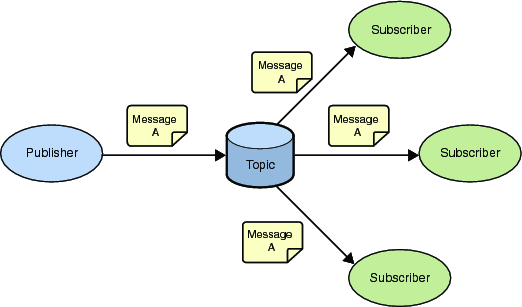
\includegraphics[scale=0.5]{cap_diseño/images/publish_subscribe}
  \caption[Estrategia \foreign{english}{publish/suscribe}: el \foreign{english}{broker} actúa como intermediario en la comunicación \foreign{english}{broadcast}.]{Estrategia \foreign{english}{publish/suscribe}: el \foreign{english}{broker} actúa como intermediario en la comunicación \foreign{english}{broadcast}. Imagen obtenida de \footnotemark.}
  \label{fig:publish-subscribe}
\end{figure}

\footnotetext{Java Messaging Service: \url{https://docs.oracle.com/cd/E19509-01/820-5892/ref_jms/index.html}}

\begin{itemize}
  \item \textbf{Ventajas}:

  \begin{itemize}
    \item \textbf{Comunicación asíncrona}: El servicio no necesita quedarse a la espera de una respuesta del servidor. Puede procesar otras operaciones hasta que se le notifique del resultado, si lo hubiera. Por otro lado, el consumidor puede ir procesándolas a su ritmo.

    \item \textbf{Escalable}: Varias instancias del mismo servicio pueden estar a la escucha de la misma cola. De esta forma, podemos aumentar la capacidad de cómputo de forma transparente a los emisores.

    \item \textbf{Desacoplamiento de los servicios}: Ni los productores ni los consumidores necesitan conocer el origen o destino de sus mensajes. Solo su formato, las colas o temas y la dirección del \foreign{english}{broker}.

    \item \textbf{Envío garantizado de mensajes}: El \foreign{english}{broker} garantiza que el mensaje será entregado \emph{al menos} una vez al consumidor. Reintentará el reenvío hasta que se confirme su recepción.

  \end{itemize}

  \item \textbf{Desventajas}:

  \begin{itemize}
    \item \textbf{Requisitos de infraestructura}: Utilizar un \foreign{english}{broker} de mensajería puede incrementar la dificultad de nuestros despliegues. Este puede convertirse en un punto de fallo único. Para operar de forma fiable, estos sistemas requieren de replicación. \cite{newmanBuildingMicroservicesDesigning2021}

    \item \textbf{Desacoplamiento de componentes}: Debido al alto nivel de desacoplamiento, puede resultar difícil detectar cuando el consumidor no está recibiendo los mensajes. Por ejemplo, si el emisor los está publicando en una cola equivocada. Los mensajes se acumularían en esta cola errónea y el consumidor real no recibiría nada.

    \item \textbf{Envío garantizado de mensajes}: Si se reintenta el envío del mensaje, es posible que ya lo hayamos consumido. Debemos diseñar nuestros sistemas de forma que estos mensajes duplicados sean descartados si ya han sido procesados.
  \end{itemize}
\end{itemize}

En la tabla \ref{tab:comparativa-mecanismos-comunicacion} presentamos un resumen de esta comparativa:

\begin{longtable}{|>{\centering}p{0.28\linewidth} | >{\centering}p{0.1\linewidth} | >{\centering}p{0.1\linewidth} | >{\centering}p{0.12\linewidth} | >{\centering\arraybackslash}p{0.25\linewidth} |}
  \hline
  & \textbf{RPC} & \textbf{REST} & \textbf{GraphQL} & \textbf{Broker mensajería} \\
  \hline
  \textbf{Tipo de comunicación y cardinalidad} & Dirigida (1..1) & Dirigida (1..1) & Dirigida (1..1) & Dirigida (1..1) y \foreign{english}{broadcast} (1..N) \\
  \hline
  \textbf{Acoplamiento entre componentes} & Alto & Medio & Alto & Bajo \\
  \hline
  \textbf{Interoperabilidad} & Baja & Alta & Alta & Alta\footnotemark \\
  \hline
  \textbf{Peticiones de lectura} & Sí & Sí & Sí & Sí\footnotemark \\
  \hline
  \textbf{Peticiones de escritura} & Si & Sí & No & Sí \\
  \hline
  \textbf{Comunicación síncrona} & Sí & Sí & Sí & No \\
  \hline
  \textbf{Comunicación asíncrona} & No & Sí & No & Si \\
  \hline
  \caption{Comparativa de los mecanismos de comunicación.}
  \label{tab:comparativa-mecanismos-comunicacion}
\end{longtable}

\footnotetext{Depende de si tenemos control sobre los componentes que queremos integrar.}
\footnotetext{Aunque no es el mecanismo ideal para lecturas. Se recomienda que los mensajes sean ligeros. Los otros protocolos serían más adecuados.}

Ahora describiremos qué protocolo elegimos para cada mecanismo de comunicación.

\subsection{Peticiones síncronas}

Comenzamos investigando el diseño de las peticiones síncronas. Tomemos por ejemplo la comunicación entre el servicio de monitorización (\foreign{english}{monitoring service}) y el servicio de conocimiento (\foreign{english}{knowledge service}). Recordemos que el conocimiento almacena todas las propiedades de adaptación. El resto de los servicios del nivel del bucle necesitan consultarlas y actualizarlas durante su funcionamiento. En la figura \ref{fig:monitor-knowledge-initial} representamos inicialmente ambos componentes y un conector, sin especificar de qué tipo será.

\begin{wrapfigure}{r}{0.37\linewidth}
  \centering
  \vspace{23pt}
  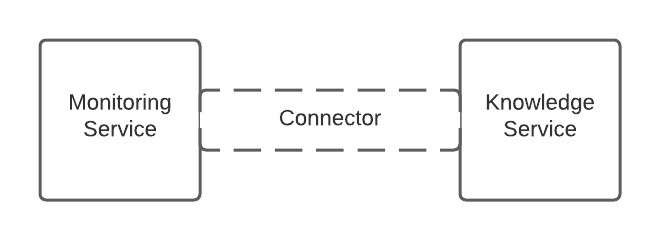
\includegraphics[scale=0.55]{cap_diseño/images/Monitor-Knowledge-Initial-Connector}
  \caption{Representación inicial del conector entre el servicio de monitorización y el de conocimiento. De momento no indica más que la necesidad de comunicación.}
  \label{fig:monitor-knowledge-initial}
  \vspace{2pt}
\end{wrapfigure}

El siguiente paso consiste en identificar qué interacciones debe existir entre ambos componentes. En este caso, el servicio de monitorización debe poder leer y actualizar el valor de las propiedades. Por tanto, existen operaciones de lectura y escritura de los datos.

De entre los cuatro tipos de conectores, pudimos descartar inmediatamente la opción de GraphQL. Se trata de un mecanismo más orientado a las consultas de datos. En nuestro caso, necesitamos ejecutar también escrituras. Aunque podríamos trabajar con dos protocolos de comunicación en paralelo, esto aumentaría la complejidad de la arquitectura. Además, el protocolo está más enfocado en consultas complejas. Como las propiedades se almacenan como pares clave - valor, sin relaciones, no lo consideramos necesario.

También descartamos emplear el \foreign{english}{broker} de mensajería. Como requerimos de lecturas de datos, nos convenía más recurrir a otros patrones. Para obtener propiedades del conocimiento, resultaba más sencillo de implementar mediante comunicación síncrona.

Finalmente, teníamos que decidir entre usar REST o RPC. Para tomar la decisión decidimos priorizar la \textbf{interoperabilidad}. Este componente estará expuesto ''hacia fuera'': expondrá su interfaz a la capa superior. Cualquier elemento que se encuentre en ella podrá contactarlo. Potencialmente, estos podrían ser desarrollados por terceros. Para maximizar la compatibilidad, descartamos entonces RPC. Este protocolo nos hubiera acoplado a una tecnología concreta y a APIs no estándares.

Nos terminamos decantando entonces por el conector REST. Implementamos ambas funciones de lectura y escritura mediante \foreign{english}{endpoints} HTTP. Su especificación se detalla a continuación en las tablas \ref{tab:especificacion-get-property} y \ref{tab:especificacion-put-property}. En ellas se incluye la operación y la ruta sobre que aplica.

\newsavebox\getpropertyrequestbox
\begin{lrbox}{\getpropertyrequestbox}
  \begin{minipage}[t]{1in}
    \begin{verbatim}
Request:
HTTP GET property/currentTemperature

Response: 200 Ok
{
  value: {
    "Value":16.79,
    "Unit": "Celsius",
    "ProbeId":"c02234d3-329c-4b4d-aee0-d220dc25276b",
    "DateTime":"2022-01-15T18:19:38.5231231Z"
  },
  lastModification: "2022-01-15T18:19:39.123213Z"
}
    \end{verbatim}
  \end{minipage}
\end{lrbox}

\begin{longtable}{|m{3.4cm}|p{2.5cm}|p{1cm}|p{3cm}|}
  \hline

  \textbf{Operación HTTP} & GET & \textbf{Ruta} & property/\{\emph{propertyName}\} \\
  \hline

  \textbf{Descripción} & \multicolumn{3}{|l|}{Devuelve el valor de la propiedad, si existe.} \\
  \hline

  \textbf{Parámetros} & \emph{propertyName} & \multicolumn{2}{|m{0.55\linewidth}|}{El nombre de la propiedad que deseamos obtener. Se lee a partir de la ruta de la petición.}\\
  \hline

  \multirow{3}*{\textbf{Respuestas posibles}}
        & \textbf{Código 200 (Ok)} & \multicolumn{2}{|m{0.55\linewidth}|}{La propiedad se ha encontrado. Incluye un \foreign{english}{payload} con el siguiente esquema:

        \begin{itemize}
          \item \foreign{english}{Value}: Valor de la propiedad serializado en JSON.
          \item \emph{LastModification}: Fecha y hora de la última modificación de esta propiedad.
        \end{itemize}}\\

        \cline{2-4}

        & \textbf{Código 400 (Bad request)} & \multicolumn{2}{|m{0.55\linewidth}|}{La petición está mal formada. No concuerda con el contrato.}\\

        \cline{2-4}

        & \textbf{Código 404 (Not found)} & \multicolumn{2}{|m{0.55\linewidth}|}{No se ha encontrado ninguna propiedad con el nombre proporcionado.}\\
  \hline

  \textbf{Ejemplo} & \multicolumn{3}{|b{0.7\linewidth}|}{Petición para obtener la propiedad \emph{currentTemperature}:
  \usebox\getpropertyrequestbox} \\

  \hline

  \caption{Especificación de la operación para obtener una propiedad del servicio de conocimiento.}
  \label{tab:especificacion-get-property}
\end{longtable}

\newsavebox\putpropertyrequestbox
\begin{lrbox}{\putpropertyrequestbox}
  \begin{minipage}[t]{2in}
    \begin{verbatim}
Request:
HTTP PUT property/currentTemperature

{
  value: {
    "Value":16.79,
    "Unit": 1, // Celsius
    "ProbeId":"c02234d3-329c-4b4d-aee0-d220dc25276b",
    "DateTime":"2022-01-15T18:19:38.5231231Z"
  }
}

Response: 204 (No content)
        \end{verbatim}
  \end{minipage}
\end{lrbox}

\begin{longtable}{|m{3.4cm}|m{2.5cm}|b{1cm}|b{3cm}|}
  \hline

  \textbf{Operación HTTP} & PUT & \textbf{Ruta} & property/\{\emph{propertyName}\} \\
  \hline

  \textbf{Descripción} & \multicolumn{3}{|b{0.7\linewidth}|}{ Actualiza (o crea, si no existe) el valor de la propiedad con el nombre dado.} \\
  \hline

  \multirow{2}*{\textbf{Parámetros}}
        & \emph{propertyName} & \multicolumn{2}{|b{0.55\linewidth}|}{El nombre de la propiedad que deseamos crear o actualizar. Se lee a partir de la ruta de la petición.}\\

        \cline{2-4}

        & \emph{SetPropertyDTO} & \multicolumn{2}{|b{0.55\linewidth}|}{ Un DTO que contiene el valor a asignar en la propiedad serializado en JSON. El DTO se encuentra en el cuerpo de la petición.} \\
  \hline

  \multirow{2}*{\textbf{Respuestas posibles}}
        & \textbf{Código 204 (No content)} & \multicolumn{2}{|b{0.55\linewidth}|}{La propiedad se ha creado o actualizado correctamente. No incluye \emph{payload} en el cuerpo de la respuesta.}\\

        \cline{2-4}

        & \textbf{Código 400 (Bad request)} & \multicolumn{2}{|b{0.55\linewidth}|}{La petición está mal formada. No concuerda con el contrato.}\\
  \hline

  \textbf{Ejemplo} & \multicolumn{3}{|b{0.7\linewidth}|}{Petición para actualizar la propiedad \emph{currentTemperature} con una medición de un termómetro:
  \usebox\putpropertyrequestbox} \\

  \hline

  \caption{Especificación de la operación para actualizar o crear una propiedad del servicio de conocimiento.}
  \label{tab:especificacion-put-property}
\end{longtable}

Una vez definida la interfaz que expondrá el servicio de conocimiento, nos quedaba definir cómo se invocaría desde el servicio de monitorización. ¿Implementamos las llamadas manualmente con un cliente HTTP? Aunque no sería muy complicado, tendríamos que mantenerlo manualmente cuando evolucione el sistema. Optamos entonces por una alternativa: generar clientes a partir del estándar OpenAPI.

\subsubsection{Open API}
\label{chap:OpenAPI}

\begin{wrapfigure}{r}{0.3\linewidth}
  \vspace{5pt}
  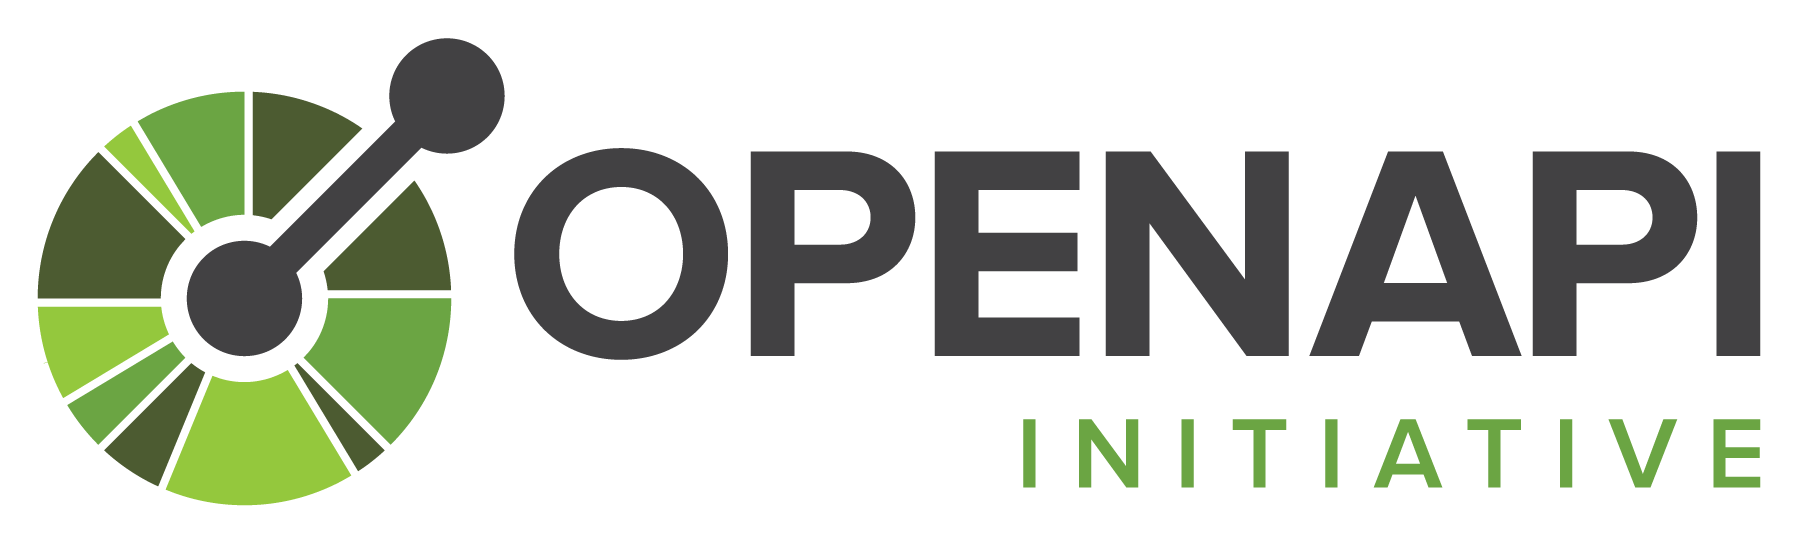
\includegraphics[scale=0.30]{cap_diseño/images/openapi-logo}
  \centering
  \vspace{5pt}
\end{wrapfigure}

OpenAPI\footnote{Página oficial: \url{https://www.openapis.org/}} es un lenguaje estándar para describir APIs REST. Nos permite especificar de forma estructurada las operaciones que ofrece un servicio, manteniéndose agnóstico a su implementación. Esta descripción ayuda tanto a humanos como a computadoras a descubrir y utilizar las funcionalidades de la API.\cite{openapiinitiativeOpenAPISpecificationV3} La OpenAPI Initiative (OAI) dirige el proyecto bajo el manto de la Linux Foundation.

Un documento OpenAPI describe el funcionamiento de la API y el conjunto de recursos que la componen. Especifica las operaciones HTTP que se pueden ejecutar sobre estos recursos y las estructuras de datos de entrada o salida. También se incluyen los códigos de respuesta de HTTP: códigos indican al cliente el resultado de la ejecución de la operación. \cite{openapiinitiativeOpenAPISpecificationV3} Más adelante, en el fragmento \ref{ls:openapi-get}, mostraremos un ejemplo de un documento típico.

La especificación puede escribirse manualmente o puede generarse a partir de una implementación existente. Así, podemos desarrollar primero nuestro servicio en un determinado lenguaje y obtener después su descripción en OpenAPI. Además, se podrá aprovecharla en varios ámbitos del desarrollo gracias a la  \textbf{variedad de herramientas} existentes: generación de documentación, generación de casos de prueba, identificar cambios incompatibles, etc. \cite{westerveldChapterOpenAPIAPI2021}

Uno de los casos de uso más interesantes es la \textbf{generación de código}. Existen una serie de librerías\footnote{\url{https://github.com/OpenAPITools/openapi-generator}} capaces de generar clientes o servidores conforme a la especificación. Ofrecen soporte a una gran variedad de lenguajes: Java, C\#, JavaScript... En el caso del \textbf{cliente}, actúa como un proxy que nos abstrae de la lógica de comunicación con el servidor. Similar a lo ya descrito en el apartado de RPC.

Para el desarrollo de este trabajo, nos interesaba especialmente debido a las posibles diferencias tecnológicas entre microservicios. Cada uno de ellos puede implementarse utilizando distintos lenguajes o librerías dependiendo de la funcionalidad a ofrecer. Gracias a la generación de código, se podría obtener la especificación del servidor y generar los clientes o servidores en cualquiera de los lenguajes soportados.

\subsubsection{Arquitectura del conector}

Para terminar, mostramos la estructura del conector que empleamos para implementar las peticiones síncronas. Aparece en la figura \ref{fig:monitor-knowledge-connector-architecture}. Esta muestra como el servicio de monitorización contacta al de conocimiento para asignarle un valor a la propiedad \emph{Temp} (temperatura).

El conector, delimitado por una línea discontinua roja, está compuesto por dos elementos: una API REST y un cliente. Los otros dos grupos representan los procesos de los servicios de monitorización y conocimiento. El servicio de monitorización se comunica con la API través del API Client. Este se despliega dentro de su proceso actuando como \emph{proxy}. En el capítulo \ref{chap:implementación} - \nameref{chap:implementación} describiremos nuestra propuesta para su implementación.

\begin{figure}[htb]
  \centering
  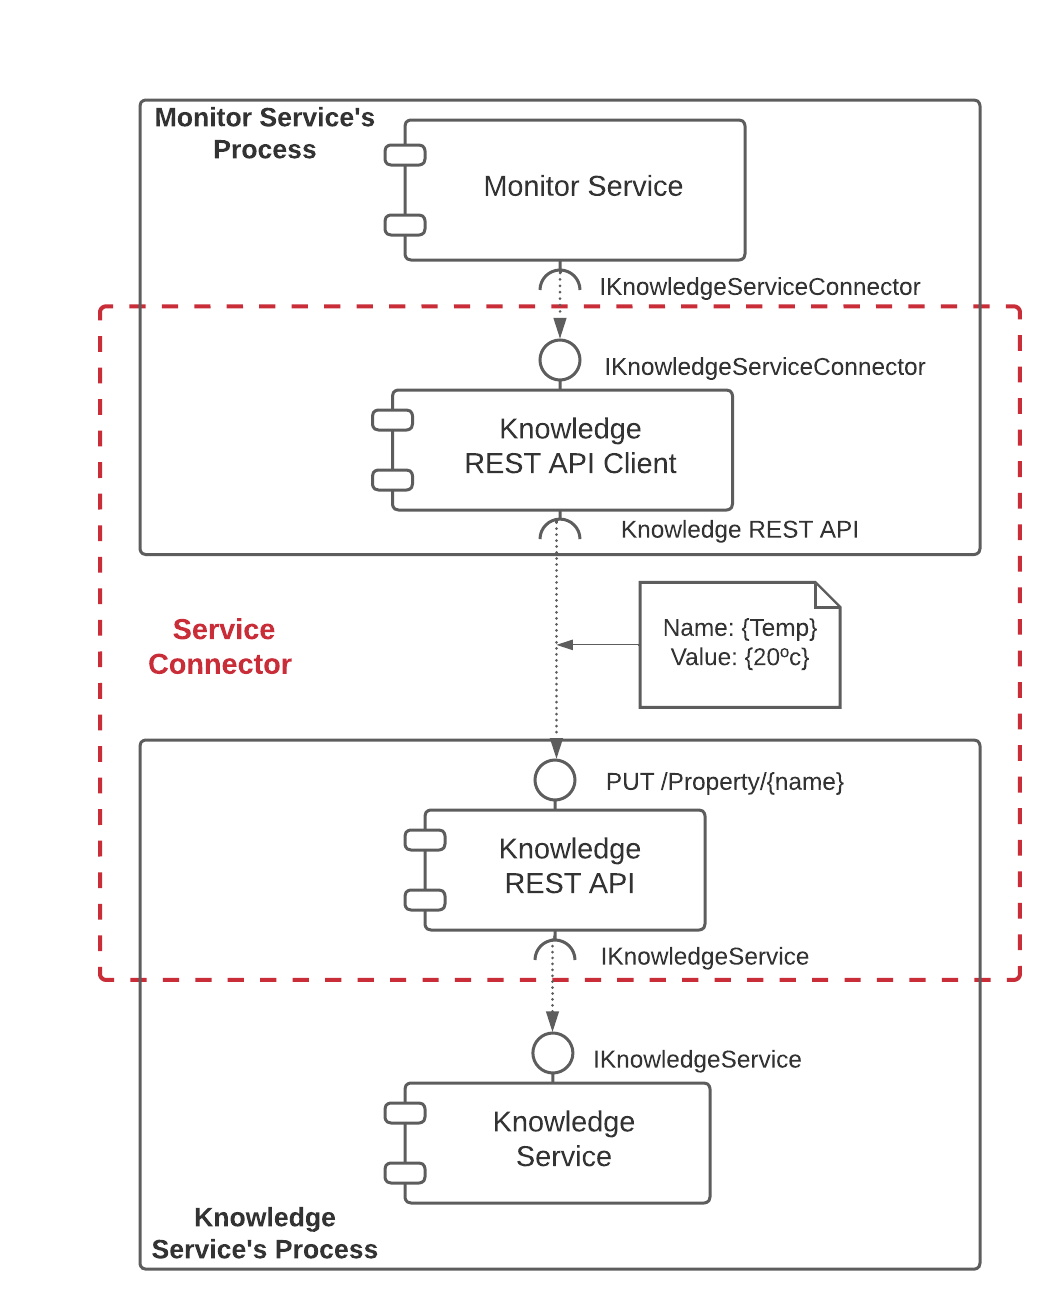
\includegraphics[scale=0.65]{cap_diseño/images/Monitor-Knowledge-Connector}
  \caption{Arquitectura del conector de peticiones síncronas.}
  \label{fig:monitor-knowledge-connector-architecture}
\end{figure}

\subsection{Notificaciones}
\label{sec:notificaciones}

\begin{wrapfigure}{l}{0.34\linewidth}
  \centering
  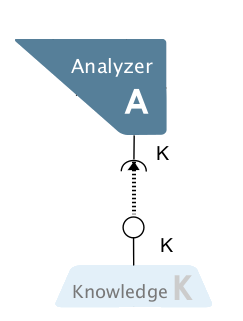
\includegraphics[scale=0.55]{cap_diseño/images/Knowledge-Analysis-Initial-Notification-Connector}
  \caption{Representación inicial del conector entre el servicio de conocimiento y el de análisis.}
  \label{fig:knowledge-analysis-notification-initial-connector}
  \vspace{-10pt}
\end{wrapfigure}

El siguiente mecanismo de comunicación que tratamos fueron las notificaciones. Recordemos que es de tipo \textbf{\foreign{english}{broadcast}}: consiste en transmitir mensajes desde un servicio a todos aquellos que pertenecen a la capa superior. Cada uno decidirá si debe procesarlo o no. Sería ideal entonces priorizar el \textbf{desacoplamiento} entre el emisor y los destinatarios.

Para estudiarla, se tomó como ejemplo la comunicación entre el servicio de conocimiento y los aquellos en el nivel del bucle. Cada vez que se modifique una propiedad de adaptación o una clave de configuración, emitirá una notificación a la capa superior. Así, por ejemplo, el servicio de análisis sabrá que debe evaluar las reglas de adaptación (figura \ref{fig:knowledge-analysis-notification-initial-connector}).

A continuación, analizamos qué tipo de conector era el más indicado. Empezamos descartando GraphQL porque es un protocolo basado en lecturas. Como el objetivo es enviar información a otros servicios, no nos servía. Respecto a RPC y REST, tampoco cumplían nuestras necesidades. Estos protocolos requerirían de conocer la dirección de todos los servicios para poder contactarlos. O, en su defecto, requeriríamos de un intermediario que los tenga registrados.

Por tanto, optamos por implementarlo usando un \foreign{english}{broker} de mensajería. Concretamente, siguiendo el patrón \textbf{\foreign{english}{publish-subscribe}}. El servicio de conocimiento publicaría el evento a través del \foreign{english}{broker}. Este evento tendrá como \foreign{english}{topic} asociado el nombre de la propiedad que ha cambiado. Así, los servicios de la capa superior podrían decidir si suscribirse o no al tipo de notificación. El \foreign{english}{broker} añadirá el mensaje en las colas de mensajería de cada uno de los suscriptores. Entonces, podrán procesarlo cuando puedan, de forma asíncrona.

En la tabla \ref{tab:especificacion-property-changed-integrationevent} mostramos la especificación del evento. Se puede apreciar que el mensaje enviado incluye la \textbf{información mínima indispensable}: el nombre de la propiedad que ha cambiado. Elegimos esta aproximación porque se trata de una comunicación asíncrona. Desde que se emite el evento hasta que se procesa, el valor de la propiedad puede haber cambiado. De esta forma, obligamos a las reglas a solicitar su valor en el momento en que se evalúen. Siempre se ejecutarán con la información actualizada.

\newsavebox\propertychangedeventbox
\begin{lrbox}{\propertychangedeventbox}
  \begin{minipage}[t]{2in}
    \begin{verbatim}
{
  "PropertyName":"Temperature"
}
        \end{verbatim}
  \end{minipage}
\end{lrbox}

\begin{table}[htb]
  \centering

  \begin{tabular}{|m{2.3cm}|p{2.5cm}|p{2.6cm}|b{1.5cm}|b{1.5cm}|}
      \hline

      \textbf{Evento} & \multicolumn{2}{|b{0.35\linewidth}|}{\emph{PropertyChangedIntegrationEvent }} & \textbf{\emph{Exchange}} & \emph{AdaptionLoop.Knowledge}  \\
      \hline

      \textbf{Descripción} & \multicolumn{4}{|b{0.6\linewidth}|}{Evento de integración que notifica sobre el cambio de una propiedad adaptación.} \\
      \hline

      \textbf{Propiedades}
            & \emph{propertyName} & \multicolumn{3}{|b{0.6\linewidth}|}{Nombre de la propiedad que ha cambiado.} \\
      \hline

      \textbf{Ejemplo} & \multicolumn{4}{|b{0.7\linewidth}|}{Evento que notifica del cambio de la propiedad \emph{Temperature}:\linebreak
      \usebox\propertychangedeventbox} \\

      \hline
  \end{tabular}

  \caption{Especificación del evento que notifica sobre el cambio de una propiedad del conocimiento.}
  \label{tab:especificacion-property-changed-integrationevent}
\end{table}

\subsubsection{AsyncAPI}

\begin{wrapfigure}{l}{0.25\linewidth}
  \vspace{15pt}
  
\includegraphics[scale=0.5]{cap_diseño/images/asyncapilogo}
  \centering
  \vspace{5pt}
\end{wrapfigure}

Para describir el evento, investigamos si existía algún estándar equivalente a OpenAPI. Y así es, se llama AsyncAPI\footnote{Página oficial: \url{https://www.asyncapi.com/}}. Por desgracia, se encuentra en fases tempranas de su desarrollo. No ha alcanzado todavía el grado de madurez e implantación que tiene su homólogo. Por ejemplo, no cuenta un catálogo muy extenso de generadores de código. Tampoco podemos extraer la especificación a partir de una implementación existente.

Aun así, lo emplearemos para describir manualmente nuestros eventos en un formato estándar. En el fragmento \ref{ls:asyncapi-propertychanged-integrationevent} presentamos la especificación del mensaje de la tabla \ref{tab:especificacion-property-changed-integrationevent}. Podemos apreciar similitudes con la especificación OpenAPI (por ejemplo, en el fragmento \ref{ls:openapi-get}). Figuran tanto la estructura del mensaje como su documentación. La mayor diferencia es la mención del canal (el \foreign{english}{exchange}  en nuestro caso) y el método (\foreign{english}{subscribe}). Esto indica que los consumidores podrán suscribirse a este evento a partir de este canal.

\pagebreak

\begin{lstlisting}[style=yaml,caption={Especificación del evento de integración \emph{PropertyChangedIntegrationEvent} en el lenguaje AsyncAPI.},captionpos=b, label=ls:asyncapi-propertychanged-integrationevent]
asyncapi: 2.4.0
info:
  title: Knowledge Service
  version: 1.0.0
  description: This service contains all the adaptation properties to inform the different stages of the loop.
channels:
  AdaptionLoop.Knowledge:
    subscribe:
      message:
        $ref: '#/components/messages/PropertyChangedIntegrationEvent'
components:
  messages:
    PropertyChangedIntegrationEvent:
      description:
        - Integration event notifying about a change in an adaption property.
      payload:
        type: object
        properties:
          propertyName:
            type: string
            description: The name of the property that changed
\end{lstlisting}

\subsubsection{Arquitectura del conector}

Para implementar este mecanismo, nuestro conector estará compuesto por tres elementos: un \textbf{publicador}, el \textbf{\foreign{english}{broker}} y un \textbf{consumidor}. Pongamos por ejemplo que el servicio de conocimiento recibe una petición para actualizar una propiedad. Si esta actualización se lleva a cabo, deberá propagar el evento a través del publicador. Este enviará el mensaje al \foreign{english}{broker} a un \foreign{english}{exchange} determinado.

El \foreign{english}{broker}, que conoce todos los suscriptores, lo añadirá en la cola de mensajería de cada uno de ellos. Sus consumidores, desplegados en cada servicio suscriptor, serán notificados del nuevo mensaje y lo procesarán en cuanto puedan. En la figura \ref{fig:knowledge-analyisis-connector-architecture} mostramos la estructura de este nuevo conector.

\begin{figure}[h!]
  \centering
  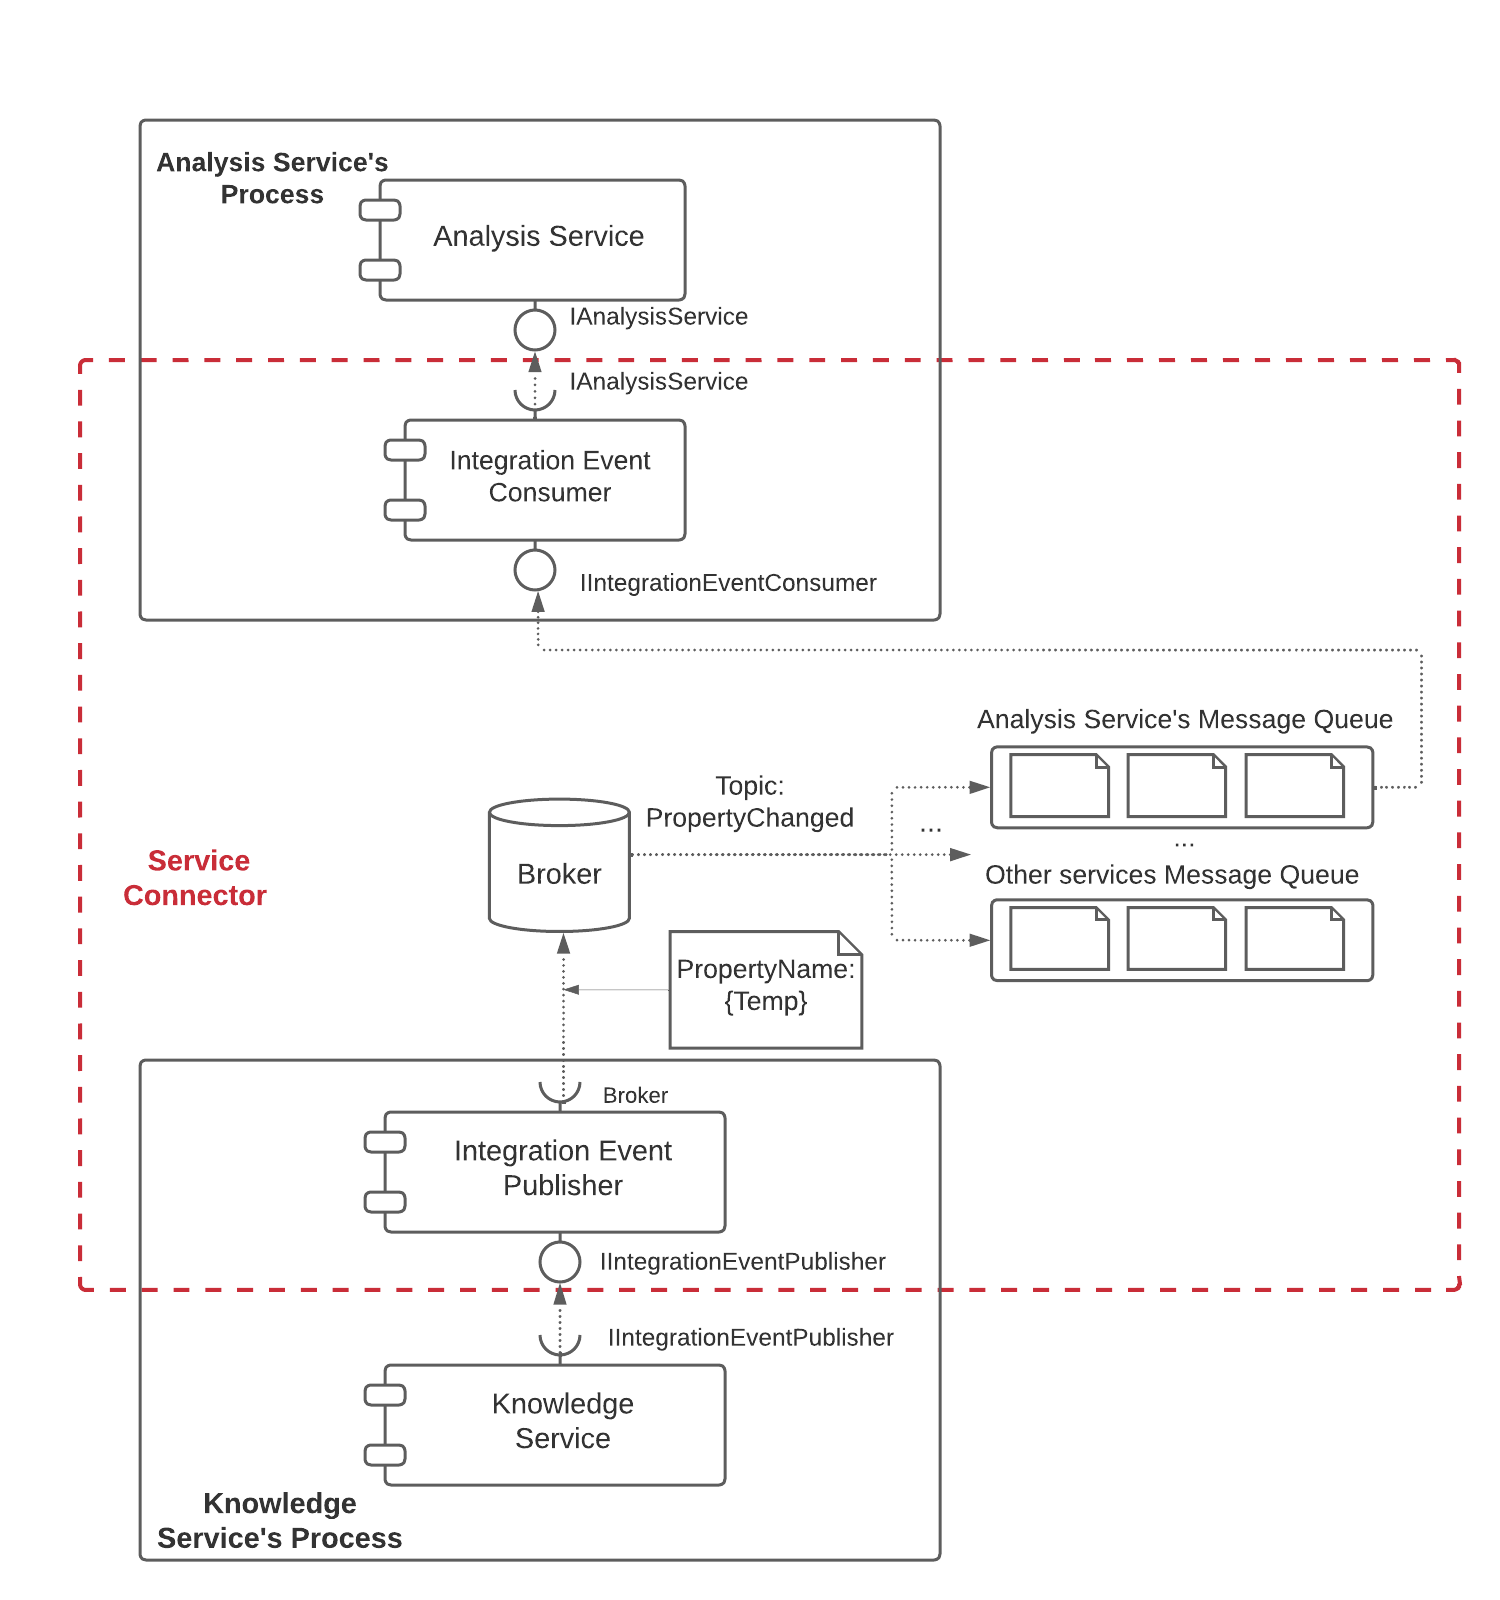
\includegraphics[scale=0.6]{cap_diseño/images/Knowledge-Analysis-Connector}
  \caption{Arquitectura del conector para notificaciones mediante un \foreign{english}{broker} de mensajería.}
  \label{fig:knowledge-analyisis-connector-architecture}
\end{figure}

\subsection{Peticiones asíncronas}

El mecanismo de comunicación restante son las \textbf{peticiones asíncronas}. Se trata de peticiones de trabajo que un microservicio envía a otro o a sí mismo. Es ideal para procesos costosos, que el destinatario podrá procesar de forma asíncrona. Ambos servicios deberán encontrarse en el mismo nivel de la jerarquía. En nuestra arquitectura tenemos dos casos que requieren de este patrón: la comunicación entre el módulo de análisis y el planificador; y aquella entre el planificador y el ejecutor. Nos centraremos en el primero (figura \ref{fig:analyisis-planner-async-request-initial-connector}).

\begin{figure}[H]
  \centering
  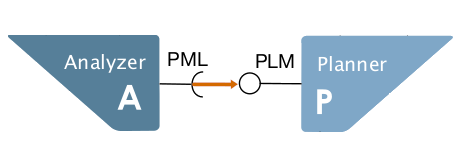
\includegraphics[scale=0.7]{cap_diseño/images/Analysis-Planner-Initial-Async-Request-Connector}
  \caption{Representación inicial del conector entre el servicio de análisis y el planificador.}
  \label{fig:analyisis-planner-async-request-initial-connector}
\end{figure}

Cuando se evalúan las reglas de adaptación, si alguna de ellas se ejecuta, propone un cambio en la configuración del sistema. Como estos servicios están en una capa superior a la del bucle, se lo transmiten al servicio de análisis mediante una petición síncrona. El módulo de análisis recibirá esta propuesta y se la enviará al planificador mediante una petición asíncrona. Podríamos haberla enviado directamente al servicio de planificación, pero preferimos que no se acoplen a un servicio adicional.

A la hora de escoger el tipo de conector, el razonamiento fue muy similar al empleado en las notificaciones. Optamos por implementarlas usando un \foreign{english}{broker} de mensajería. En este caso, empleando el patrón de \textbf{colas de trabajo}. Los \textbf{\foreign{english}{workers}} o trabajadores cuentan con una \textbf{cola de mensajería específica para las peticiones de trabajo}. El publicador la conoce y, a través del \foreign{english}{broker}, envía los mensajes directamente a ella. Los trabajadores los irán recuperando y procesando en cuanto puedan.

En la tabla \ref{tab:especificacion-system-configuration-change-request} presentamos la especificación de la petición asíncrona para solicitar un cambio de configuración en el sistema. Vemos que es muy similar a \ref{tab:especificacion-property-changed-integrationevent}. La principal diferencia es que esta incluye mucha más información que el evento. Esto es debido a que tiene más en común con una petición síncrona. El planificador recibirá todos los parámetros que necesita para ejecutar la petición. Aun así, en el momento de ejecución deberá verificar con el conocimiento que algunos de estos no hayan cambiado.

\newsavebox\systemconfigurationchangerequestbox
\begin{lrbox}{\systemconfigurationchangerequestbox}
  \begin{minipage}[t]{2in}
    \begin{verbatim}
{
  "Timestamp": "2022-06-19T16:38:30.6092751Z",
  "Symptoms":[
    {
      "Name": "temperature-lesser-than-cold-threshold",
      "Value": "true"
    }
  ],
  "ConfigurationRequests":  [
    {
      "ServiceName": "Climatisation.AirConditioner.Service",
      "IsDeployed": true,
      "ConfigurationProperties": [
        {
          "Name": "Mode",
          "Value": "Heating"
        }
      ],
      "Bindings": []
    }
  ]
}
        \end{verbatim}
  \end{minipage}
\end{lrbox}

\begin{longtable}{|m{2cm}|m{2.3cm}|m{10cm}|b{0.85cm}|b{2.75cm}|}
  \hline

  \textbf{Nombre} & \multicolumn{2}{|b{0.37\linewidth}|}{\emph{SystemConfigurationChangeRequest}} & \textbf{Cola} & \emph{AdaptionLoop.Planification.Requests}  \\
  \hline

  \textbf{Descripción} & \multicolumn{4}{|b{0.82\linewidth}|}{Petición que representa una propuesta de cambio de la configuración del sistema.} \\
  \hline

  \textbf{Propiedades}
    & \emph{Timestamp} & \multicolumn{3}{|m{0.67\linewidth}|}{Fecha y hora de la petición de cambio.} \\
    \cline{2-5}
    & \emph{Symptoms} & \multicolumn{3}{|m{0.67\linewidth}|}{Colección de síntomas que la han desencadenado.} \\
    \cline{2-5}
    & \emph{Configuration Requests} & \multicolumn{3}{|m{0.67\linewidth}|}{Colección peticiones de configuración de la propuesta de cambio.

    Cada una de estas está compuesta por:
    \begin{itemize}
      \item \textbf{\emph{ServiceName}}: Identificador del servicio cuya configuración queremos cambiar.
      \item \textbf{\emph{IsDeployed}}: Indica si el servicio debe estar desplegado o no en la siguiente configuración.
      \item \textbf{\emph{Bindings}}: Colección de conexiones que indican a qué otros servicios debe estar conectado (o no) en la siguiente configuración.
      \item \textbf{\emph{ConfigurationProperties}}: Colección de pares clave-valor que representan valores de su configuración que queremos actualizar.
    \end{itemize}} \\
  \hline

  \textbf{Ejemplo} & \multicolumn{4}{|b{0.82\linewidth}|}{Solicitud de cambio del modo de un aire acondicionado a modo calefacción (\emph{heating}). Los síntomas indican que fue desencadenada porque la temperatura era menor que un umbral determinado:\linebreak
  \usebox\systemconfigurationchangerequestbox} \\

  \hline

  \caption{Especificación de una petición de cambio de configuración del sistema.}
  \label{tab:especificacion-system-configuration-change-request}
\end{longtable}

\subsubsection{AsyncAPI}

Respecto a la especificación con AsyncAPI, las peticiones asíncronas no están soportadas todavía. A fecha de la redacción, el grupo se encuentra estudiando cómo implementarlas\footnote{Discusión disponible en: \url{https://github.com/asyncapi/spec/pull/594}}. Como mencionamos anteriormente, el estándar todavía se encuentra en desarrollo. Su inclusión está propuesta para la versión \texttt{3.0.0} de la especificación.

\subsubsection{Arquitectura del conector}

La arquitectura de este mecanismo es muy similar a la de las notificaciones. Está compuesta también por tres elementos: un \textbf{publicador}, el \textbf{\foreign{english}{broker}} y un \textbf{consumidor}. Pongamos por ejemplo que el servicio de análisis recibe una petición síncrona para cambiar el estado del sistema. Este servicio deberá traducirla a una petición asíncrona y enviarla a través del publicador. A su vez, este enviará el mensaje al \foreign{english}{broker} dirigido a una cola determinada.

El \foreign{english}{broker} simplemente lo añadirá a la cola especificada. Las instancias del planificador serán notificadas del nuevo mensaje y una de ellas lo procesará en cuanto puedan. En la figura \ref{fig:async-request-connector-architecture} mostramos la estructura de este último conector.

\begin{figure}[h!]
  \centering
  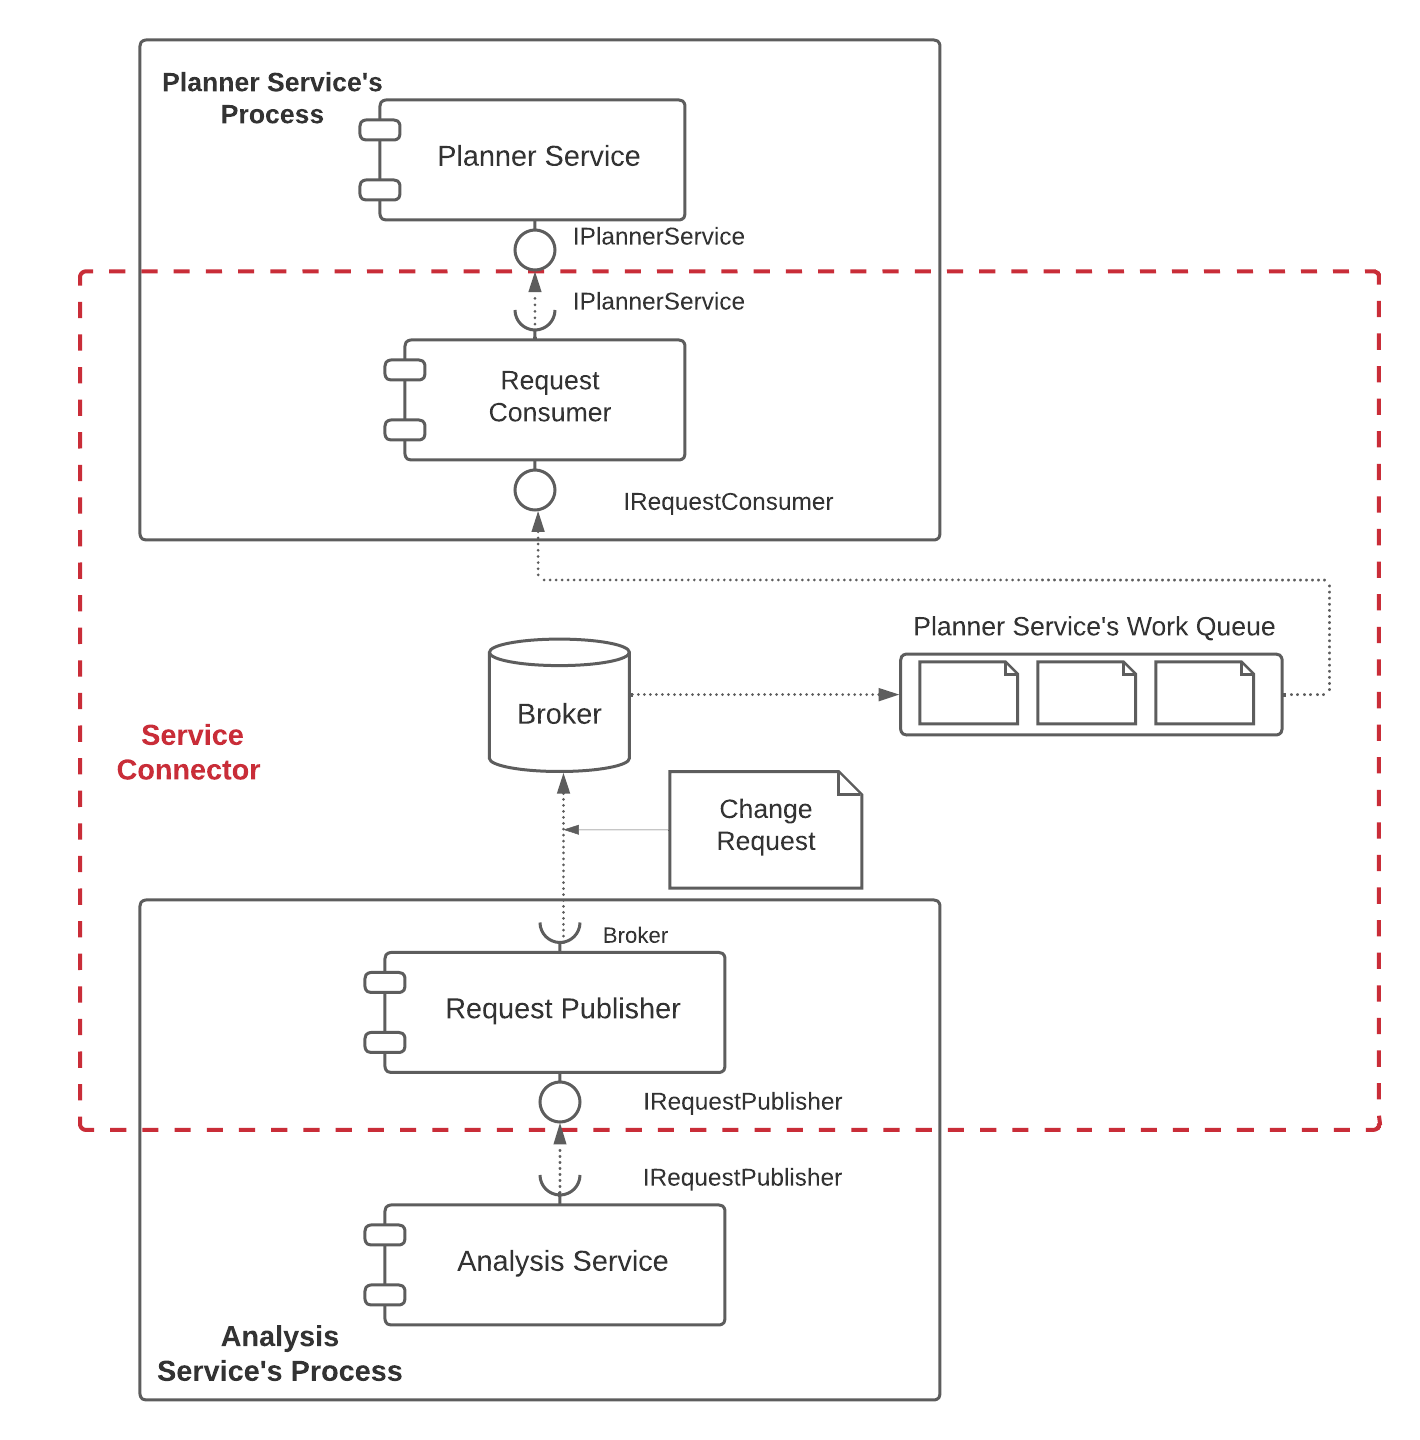
\includegraphics[scale=0.60]{cap_diseño/images/Async-Request-Connector-Architecture}
  \caption{Arquitectura del conector para peticiones asíncronas mediante un \foreign{english}{broker} de mensajería.}
  \label{fig:async-request-connector-architecture}
\end{figure}

\pagebreak

\section{Propuesta arquitectónica}

Una vez definidos los componentes y sus conectores, podemos completar nuestra propuesta arquitectónica (figura \ref{fig:arquitectura-sistema}). En esta propuesta inicial, cada componente individual representa un tipo de microservicio distinto. Un caso aparte son las sondas y efectores, que pueden desplegarse como parte del recuso manejado.

Por otro lado, los conectores entre ellos están representados mediante distintos tipos de flecha. Podemos comprobar que todas las comunicaciones respetan la jerarquía descrita en la figura \ref{fig:clean-mapek-architecture}. Los servicios de un nivel superior contactan con aquellos en la capa inmediatamente inferior mediante peticiones síncronas. Los de una capa inferior, con los de la inmediatamente superior a través de notificaciones. Y, finalmente, los de una misma capa mediante peticiones asíncronas. Las APIs que usarán para comunicarse las describimos en detalle en el anexo \ref{anx:apis} - \nameref{anx:apis}.

\begin{figure}[h!]
  \hspace{-1cm}
  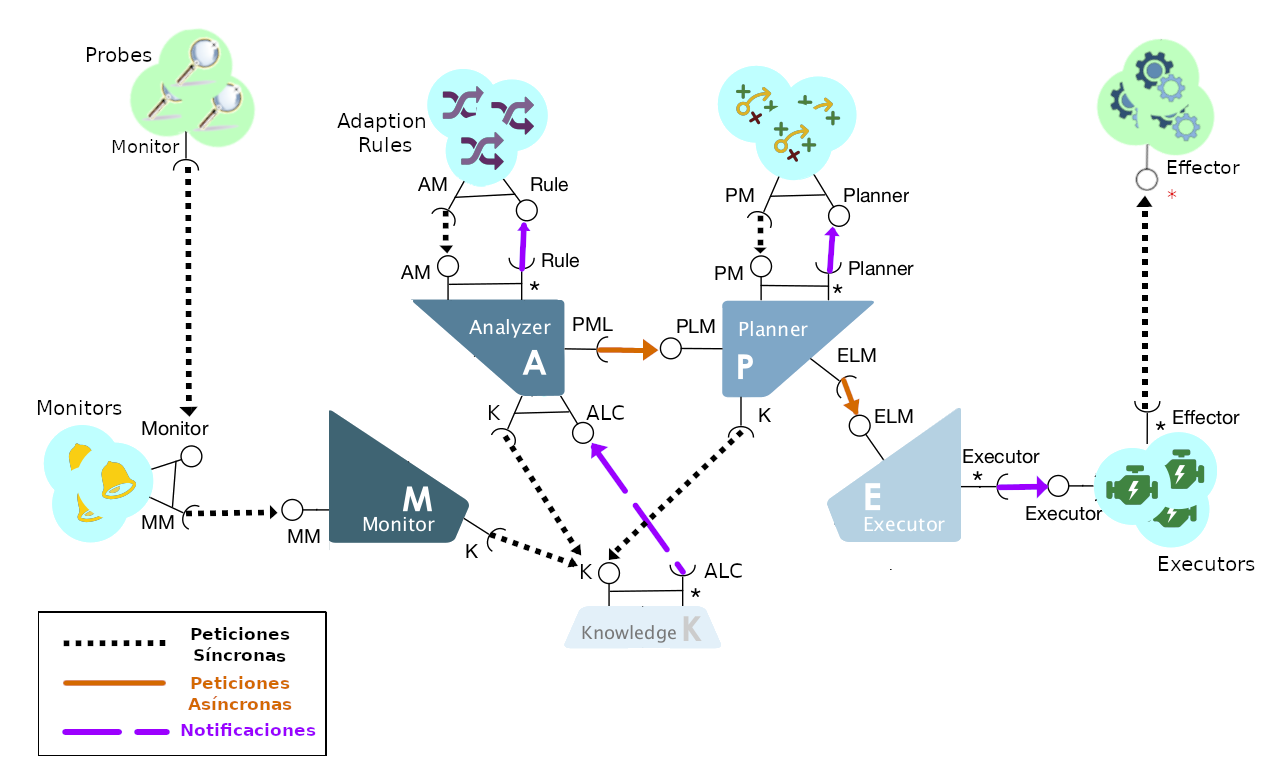
\includegraphics[scale=0.5]{cap_diseño/images/arquitectura}
  \caption{Propuesta arquitectónica inicial del bucle MAPE-K distribuido.}
  \label{fig:arquitectura-sistema}
\end{figure}
